%! TEX program = xelatex
\documentclass{report}
% provides basic settings for ctex document
\usepackage[UTF8, heading=true]{ctex}
\usepackage{fancyhdr}
\usepackage{tocloft}
\usepackage[margin=1in]{geometry}
\usepackage{metalogo}                   % \XeLaTeX
\usepackage{float}                      % figure H flag
\usepackage{microtype}                  % break long words
\usepackage[hidelinks]{hyperref}
\usepackage{tabularx}
\usepackage{amsmath}
\usepackage{lmodern}                    % allow fonts to scale
\usepackage{placeins}
\usepackage{multirow}                   % multirow, multicolumn support
\usepackage{booktabs}                   % toprule, cmidrule support
\usepackage{caption}

% make chapter stay in the same page
%\makeatletter
%\renewcommand\chapter{\thispagestyle{plain}%
%\global\@topnum\z@
%\@afterindentfalse
%\secdef\@chapter\@schapter}
%\makeatother

\fancyhead{}
\renewcommand{\sectionmark}[1]{\markleft{#1}}
\renewcommand{\partmark}[1]{\markright{#1}}
\lhead{\leftmark}
\rhead{\rightmark}
% see $(texdoc ctex) for details
\ctexset{
    chapter = {
        format += \flushleft,
        number = \arabic{chapter},
    },
    section = {
        format += \flushleft,
    },
    appendix = {
        number = \Alph{chapter},
        name = {附录},
    },
}

\pagestyle{fancy}

%\setlength\cftaftertoctitleskip{2em}

% provides code input support
\usepackage{xparse}                     % newcommand multiple optional arguments
\usepackage{listings}                   % code
\usepackage{fontspec}
\usepackage{lmodern}

%\newfontfamily\codeF{Fira Code}

\setmonofont[
    Contextuals={Alternate},
    ItalicFont = Fira Code      % to avoid font warning
]{Fira Code}

% usage: \inputCode{[language] <path>}
% if language is not explicitly set, it's defaulted to c
\DeclareDocumentCommand{\inputCode}{ O{c} m }{
    {
        \lstinputlisting[
            basicstyle=\small\ttfamily,
            language={#1},
            tabsize=4,
            showstringspaces=false,
            breaklines=true,
            frame=shadowbox,
            framexleftmargin=10mm,
            rulesepcolor=\color{black},
            numbers=left,
            xleftmargin=4em,
        ]{#2}
    }
}

\DeclareDocumentCommand{\inputCodeSetLanguage}{ m }{
    \lstset{
        basicstyle=\small\ttfamily,
        language={#1},
        tabsize=4,
        showstringspaces=false,
        breaklines=true,
        frame=shadowbox,
        framexleftmargin=10mm,
        rulesepcolor=\color{black},
        numbers=left,
        xleftmargin=4em,
    }
}


\usepackage{xparse}
\usepackage{tcolorbox}
\usepackage{mdframed}

\tcbuselibrary{breakable}
\NewDocumentCommand{\exercise}{ m +m }{
    {
        \edef\originalParIndent{\the\parindent}
        \begin{tcolorbox}[breakable,arc=0mm,boxrule=0.4pt]
            \setlength{\parindent}{\originalParIndent}
            \noindent
            \textbf{\large Exercise #1}
            \indent
            #2
        \end{tcolorbox}
    }
}

% environment style of exercise, to feed special requirements
\NewDocumentEnvironment{exerciseEnv}{m}{
    \edef\originalParIndent{\the\parindent}
    \begin{tcolorbox}[breakable,arc=0mm,boxrule=0.4pt]
        \setlength{\parindent}{\originalParIndent}
        \noindent
        \textbf{\large Exercise #1}
        \indent
} {
    \end{tcolorbox}
}

\NewDocumentEnvironment{questionEnv}{}{
    \edef\originalParIndent{\the\parindent}
    \begin{tcolorbox}[breakable,arc=0mm,boxrule=0.4pt]
        \setlength{\parindent}{\originalParIndent}
        \noindent
        \textbf{\large Question}
        \indent
} {
    \end{tcolorbox}
}

% a raised rule
\NewDocumentCommand{\raisedrule}{ O{0em} m }{\leaders\hbox{\rule[#1]{1pt}{#2}}\hfill}

\NewDocumentEnvironment{exerciseSolution}{m}{
    {\noindent \textbf{\large Exercise #1 实验过程 \raisedrule[0.3em]{0.6pt}}}
} {
    \par
    {\noindent \textbf{\large \raisedrule[0.3em]{0.6pt} Exercise #1 实验过程}}
    \vspace{1em}
}

\NewDocumentEnvironment{answer}{}{
    {\noindent \textbf{\large Answer \raisedrule[0.3em]{0.6pt}}}
} {
    \par
    {\noindent \textbf{\large \raisedrule[0.3em]{0.6pt} Answer}}
    \vspace{1em}
}



%%%%%%%%%%%%%%%%%%%%%%%%%%%%%%%%
\graphicspath{{./res/}}

% report content %%%%%%%%%%%%
%%%%%%%%%%%%%%%%%%%%%%%%%%%%%
\begin{document}

% cover page
\begin{titlepage}
    \addtolength{\topmargin}{1cm}
    \centering
    
\includegraphics[width=0.6\textwidth]{hust.jpg}\par
    \vspace{0.5cm}
    {\Huge \heiti 操作系统课程设计报告}\par
    \vspace{10cm}
    {
        \large
        \begin{tabular}{r m{8em}}
            \makebox[6em][s]{学生姓名}:& 胡思勖 \\ \cline{2-2}
            %\makebox[6em][s]{学生姓名}:& 陈志浩 \\ \cline{2-2}
            %\makebox[6em][s]{学生姓名}:& 黄志强\\ \cline{2-2}
            \makebox[6em][s]{学号}:& U201514898\\ \cline{2-2}
            %\makebox[6em][s]{学号}:& U201514893\\ \cline{2-2}
            %\makebox[6em][s]{学号}:& U201514896\\ \cline{2-2}
            \makebox[6em][s]{专业}:& 计算机科学与技术\\ \cline{2-2}
            \makebox[6em][s]{班级}:& 计卓1501\\ \cline{2-2}
            \makebox[6em][s]{指导教师}:& 张杰 \\ \cline{2-2}
        \end{tabular}
    }
    \vfill
    2018-03-03
\end{titlepage}

\setcounter{tocdepth}{1}
\pagenumbering{Roman}
\tableofcontents

\newpage
\pagenumbering{arabic}
\setcounter{page}{1}



% chapter 1
\chapter{Booting a PC}
\label{cha:booting_a_pc}

\section{PC Bootstrap}
\par 这一部分主要介绍了x86语言以及PC的启动过程,并让我们熟悉了QEMU和GDB的调试方法。

\subsection{Getting Started with x86 assembly}
\par 通过阅读\emph{PC Assembly Language Book}\footnote{\url{https://pdos.csail.mit.edu/6.828/2017/readings/pcasm-book.pdf}}来学习x86的语法。注意这本书值使用的NASM汇编,但是实验中使用的是GNU的AT\&T语法。



% chapater 2
\chapter{基于pthread的形态学图像处理}
\section{实验目的与要求}
\begin{itemize}
    \item 掌握使用pthread的基本的并行编程设计方法以及调优方法;
    \item 掌握并行编程中基本的数据分块以及任务分解的方法。
    \item 使用pthread实现并行的形态学图像处理。
    \item 简要分析以及总结处理的结果。
\end{itemize}

\section{算法描述}
\par 使用多个线程对于一个图像进行蚀刻以及膨胀的算法如下,算法为一个线程的流程,而有多个这样的线程同时进行。
\begin{simpleAlgorithm}{pthread并行处理算法(一个线程)}
    \Procedure{PthreadParallel}{$blocks$}
    \While{true}
        \State lock\((blocks)\)
        \State get first block \(blk\) from \(blocks\)
        \If{\(blocks\).empty()}
            \State unlock\((blocks)\)
            \State \Return
        \EndIf
        \State unlock\((blocks)\)
        \State \Call{ErodeAndDilate}{$blk, kernel_e, kernel_d$}
    \EndWhile
    \EndProcedure
\end{simpleAlgorithm}
\par 算法中,\(blocks\)参数为一个工作队列,队列中的工作为原预处理过后的图片的子图片。在每个线程的每个循环中,首先锁住队列,从队列中获取一个子图片\(blk\)、解锁队列然后使用上一章中的ErodeAndDilate过程进行处理。如果\(blocks\)中没有子图片,说明处理完成,则此线程退出。
\par 主线程的流程如图\ref{fig:pthreadMain}所示。在进行预处理过后启动多个线程,然后等待所有线程竞争子图像、处理然后结束即可,最后保存处理的结果即可。
\begin{figure}[htpb]
    \centering
    
\includegraphics[width=0.95\linewidth]{pthreadMain.png}
    \caption{主线程流程}
    \label{fig:pthreadMain}
\end{figure}

\par 由于是使用pthread的并行算法,每一个线程处理一个部分,因此首先需要将数据分块(即分为算法中的\(blocks\))。分块方式如图\ref{fig:partition}所示。每块大小一样,在边缘部分如果块大小不符则按照原图的边缘进行裁减。因此,在进行处理时需要对于边缘部分进行考虑。
\begin{figure}[htpb]
    \centering
    
\includegraphics[width=0.76\linewidth]{partition.png}
    \caption{分块方法}
    \label{fig:partition}
\end{figure}

\section{实验方案}
\par 所有的开发与运行环境见附录\ref{cha:env},表\ref{tab:env},此后实验的开发与运行环境均相同,不再赘述。根据算法描述、分块方法以及主线程的流程编写程序并运行,然后观察结果并与串行的程序比较。经过多轮的比较以及参数调试后得出一个较好的效果。

\section{实验结果与分析}
\par 功能上,程序处理后的图片与串行处理后的图片一致,此处不再给出。4线程,分块大小为128的情况下程序的运行时间如图\ref{fig:pthreadOutput}所示。在4个线程的情况下,运行三次的平均运行时间为11.7s,相比于串行算法,程序的加速比为\(44.2\div 11.7 = 3.77\),已经十分接近理想加速比4。
\begin{figure}[htpb]
    \centering
    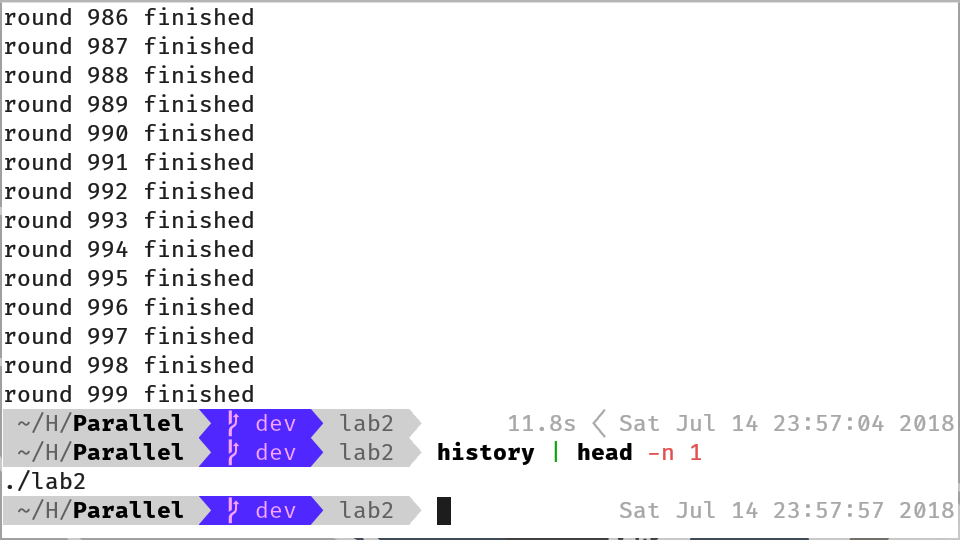
\includegraphics[width=0.9\linewidth]{pthreadOutput.png}
    \caption{pthread程序运行时间}
    \label{fig:pthreadOutput}
\end{figure}

\par 经过8组、每组3次的测试,加速比随线程变化的曲线如图\ref{fig:pthreadTrend}所示。可以看出,在线程数为1\textasciitilde 4时加速比随着线程数几乎呈线性变化,而在线程数为1时加速比为1.006,overhead所占用的时间几乎可以不计。在线程数达到4时由于物理内核已经被占满,因此后面加速比不再增加,随着线程数量的进一步增大,由于线程调度的开销,因此程序的加速比不再增加,反而有所下降。
\begin{figure}[htpb]
    \centering
    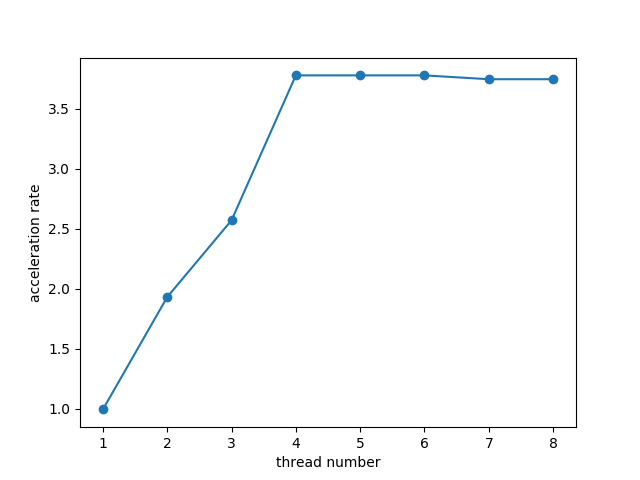
\includegraphics[width=0.8\linewidth]{pthreadTrend.png}
    \caption{加速比随线程数变化}
    \label{fig:pthreadTrend}
\end{figure}

\par 对于分块大小而言,加速比随着分块大小的变化如图\ref{fig:pthreadTrend2}所示,在分块大小较小时,加速比随着分块大小的变化并不大,只在分块大小过小时由于线程调度导致一点性能开销。当分块大小大于原图的一半时总时间则取决于分到最大分块线程所用的时间,因此在这个区间内性能随分块大小呈下降趋势。
\begin{figure}[htpb]
    \centering
    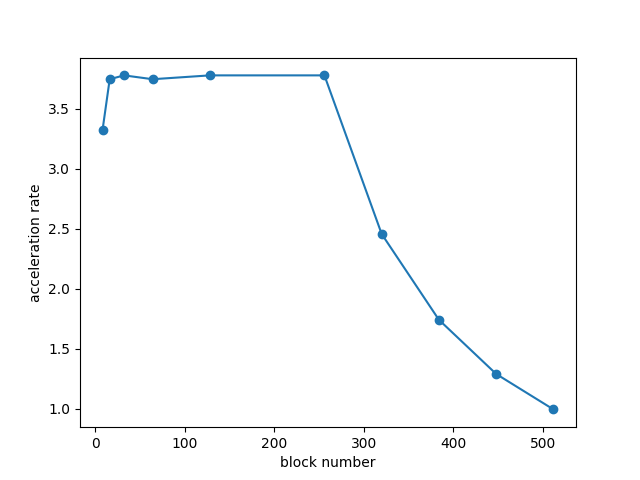
\includegraphics[width=0.8\linewidth]{pthreadTrend2.png}
    \caption{加速比随分块大小变化}
    \label{fig:pthreadTrend2}
\end{figure}




% chapater 3
\chapter{基于OpenMP的形态学图像处理}
\section{实验目的与要求}
\begin{enumerate}
    \item 掌握使用OpenMP进行并行编程设计和性能优化的基本原理和方法
    \item 使用OpenMP实现形态图像处理操作的并行算法
    \item 对程序执行结果进行简单的分析和总结
    \item 将其与Lab2的结果进行比较
\end{enumerate}

\section{算法描述}
\par 使用OpenMP进行并行计算与使用pthread进行并行计算的算法原理几乎一样,只不过OpenMP由编译器进行底层实现,使用for循环进行包装,且主线程不是空闲的,而是也参与计算。而pthread则需要人工进行底层的编写。使用OpenMP的关键部分代码如下:
\inputCodeSetLanguage{c++}
\begin{lstlisting}
#pragma omp parallel for num_threads(threadNum) schedule(dynamic, 2)
for(int i=0; i < workNum; ++i){
    // Code equvilent to calling ErodeAndDilate(blk, kernel_e, kernel_d)
}
\end{lstlisting}
\par OpenMP caluse中的schedule(dynamic, 2)将所有的人物按照2个一组进行分组,而每个线程领取一组任务、执行完成后在领取下一组可能的任务,从而避免了由于静态调度以及线程执行时间不等带来的CPU空闲。

\section{实验方案}
\par 由于算法与pthread基本相同,因此可以在pthread的实现上进行修改,将pthread中的线程竞争调度改为使用openmp directive包装的for循环,并在编译条件中去除-lpthread,加上-fopenmp即可。
\par 在运行时,通过多次调节参数并进行重复实验,得到一侧较优的参数,然后将这个参数与phtread实现进行对比,观察OpenMP实现与pthread实现的区别。

\section{实验结果与分析}
\par 功能上,OpenMP能够正确的处理图片并给出与串行处理相同的结果。性能上,使用4线程、分块大小128时程序的运行结果如图\ref{fig:ompOutput}所示。三次测试平均结果为12.63s,相对于串行程序加速比为\(44.2\div 12.63 = 3.49\),与同条件下的pthread实现比起来加速比要低不少,这是由于OpenMP需要进行环境的初始化,且其调度过程没有特别为底层实现的pthread程序优化,因此pthread实现的并行程序性能较为优秀。
\begin{figure}[htpb]
    \centering
    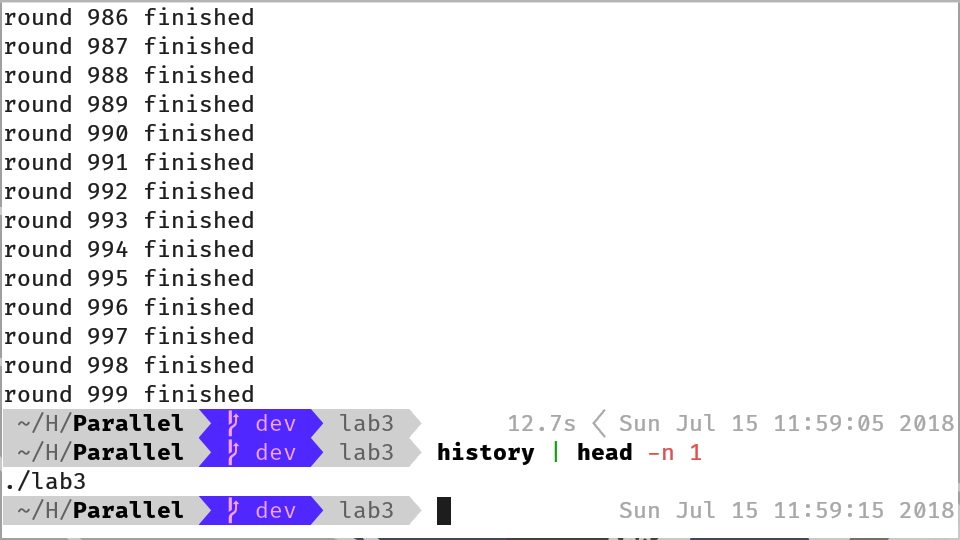
\includegraphics[width=0.9\linewidth]{ompOutput.png}
    \caption{使用OpenMP进行处理的输出}
    \label{fig:ompOutput}
\end{figure}

\par 加速比随线程数量变化如图\ref{fig:ompTrend}所示,其中实线部分为使用OpenMP的程序,而虚线部分为上述使用pthread的程序。从图中可以看出,使用OpenMP和使用pthread程序的性能随着线程数量的变化趋势是一样的,因为其算法本质上是相同的。而使用OpenMP的程序在同样的情况下总是比使用pthread的程序要慢一些,这也是由于OpenMP并不是一个针对特殊程序的调度算法,因此没有更为底层的,为特殊目的设计的pthread程序性能高,但在仅需要编写较少代码的情况下能够达到与pthread程序接近的性能说明其实现也是十分优秀的。
\begin{figure}[htpb]
    \centering
    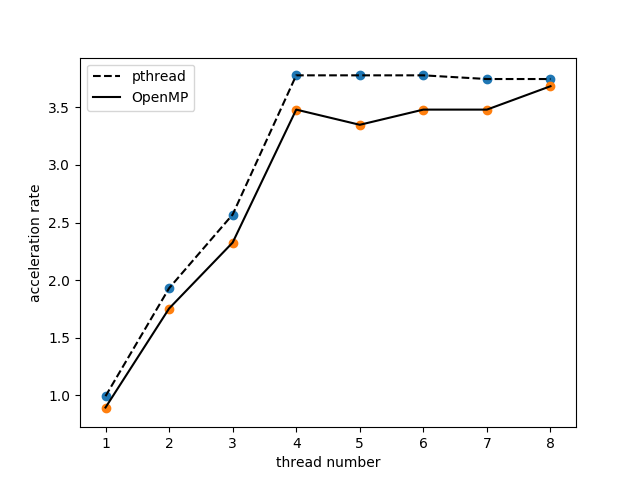
\includegraphics[width=0.8\linewidth]{ompTrend.png}
    \caption{加速比随线程数量变化}
    \label{fig:ompTrend}
\end{figure}
\par 而加速比随分块大小的变化如图\ref{fig:ompTrend2}所示,同样,实线为OpenMP实现,虚线为pthread实现。与随着线程变化的趋势一样,在同样的情况下OpenMP的性能比pthread性能低。在分块大小超过图片的1/2时更为明显,其下降趋势更为剧烈,推测是由于OpenMP的启动与初始化时间以及调度的分块引起的。
\par 从上述结果可以得出结论:在对于并行性能要求不是非常高时,使用OpenMP可以简化程序编写者的工作量,而使用pthread作出针对特定程序的并行算法则相对于OpenMP算法可以较大的提高程序的性能。
\begin{figure}[htpb]
    \centering
    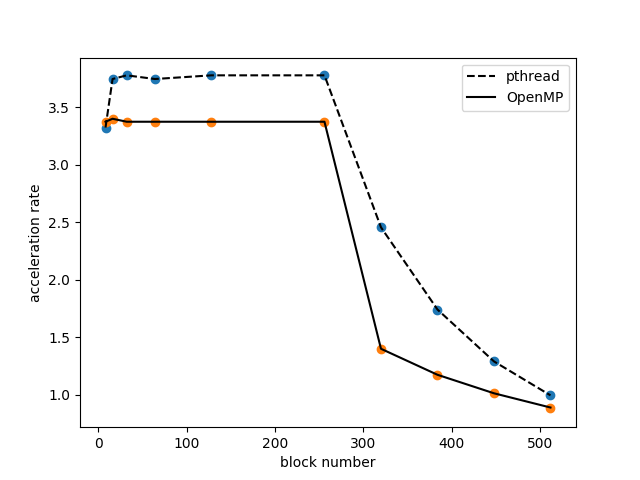
\includegraphics[width=0.8\linewidth]{ompTrend2.png}
    \caption{加速比随线分块大小变化}
    \label{fig:ompTrend2}
\end{figure}




\chapter{目标代码生成}
\label{cha:mu_biao_dai_ma_sheng_cheng_}

\section{实验设计}
\label{sec:shi_yan_she_ji_4}
\par 在生成了TAC后,剩下的部分就是目标代码生成了。在这一部分中,程序将由能力生成可以运行的MIPS指令。
\par 由于前面已经生成了三地址码,生成对应的mips指令只需将一种线性结构转换为另一种线性结构,这一部通过CodeGenerator类中的generateFinalCode完成。其中的核心部分在于寄存器的分配。可供分配的寄存器数量有限,而TAC中的临时变量一般远远超出可以分配的寄存器数量,因此需要知道那些变量不再使用,便于将其所绑定的寄存器空出给其他的变量使用。
\par 要完成这一点,需要对程序进行数据流分析,而其中的第一步则是构建程序的流图。在本实验中,使用一个ControlFlowGraph作为存储流图的数据结构,对于流图这样一个有向无环图,ControlFlowGrap采用双向邻接表的数据结构表示。对于个节点的出度使用一个矩阵,入度使用另一个,并分别建立ForwardFlow类以及BackwardFlow类作为原图的遮罩,便于图的前向遍历和方向遍历。
\par 生成最终代码的大体框架分为3步:
\begin{enumerate}
    \item 遍历CodeGenerator中的TAC指令,生成CFG。
    \item 遍历CFG,生成活跃变量表。
    \item 遍历CodeGenerator中的TAC指令,结合活跃变量表,完成最终的寄存器分配以及代码生成。
\end{enumerate}

\inputCodeSetLanguage{c++}
\par 这些步骤均在generateFinalCode中完成。活跃变量表采用\lstinline|list<map<Location,Instruction>>|的结构实现,其中,外层的list为源程序中不同的函数,每个函数有自己的CFG, 而内层的map则是对于cfg进行分析后的活跃变量表,它将变量(Location类,变量使用变量地址表示)映射到\textbf{最后一次使用它的指令}。这样,在后续的遍历过程中,只需要查找所使用的变量是否在活跃变量表中,如果在,则比对当前的指令是否与其最后一次使用的指令相同,如果相同,则说明这是最后一个使用这个变量的指令。此变量已经可以被丢弃,此后不会再被使用了。
\par 第三步执行的正是这样的工作:遍历TAC指令并决定是否丢弃用到的变量。为了减少程序的耦合度,不因为丢弃变量而干扰其他类,使用上一章中提到的DiscardValue这一伪TAC指令生成目标指令,这样解绑寄存器的策略就决定与最终用于生成目标指令的类而不是CodeGenerator这一生成TAC指令的类了。
\par 与从AST到TAC类似,为了便于程序的控制,减小各个模块之间的耦合度,采用Mips类进行最终的代码生成。由于产生的TAC指令与LLVM后端不兼容,要使用LLVM生成则过于复杂,因此使用此类直接硬编码生成MIPS指令。由于将TAC生成与最终代码的生成分离,因此可以轻易的将Mips类替换成其他类,用以生成x86, arm等一系列平台的目标代码。对于本实验中的Mips类而言,其通过不同的函数将TAC类映射到对应的Mips代码的生成方法,而Instruction类的各个子类通过虚函数重载了generateSpecific方法用于调用生成与自身TAC类相关的Mips指令,因此在CodeGenerator中只调用每个TAC指令的generateSpecific方法以及丢弃指令的generateSpecific即可生成最终的Mips代码。由于未作特别的代码优化,在Mips类中,除了特殊寄存器(如sp)保留之外,其余的空闲寄存器均是随机分配的,以达到均匀使用所有寄存器的效果。

\section{实验步骤}
\label{sec:shi_yan_bu_zou_4}
\par 作为程序流图的基础,首先构建ControlFlowGraph类,然后对于其中的mapLabels以及mapEdges方法进行编写,对于普通TAC指令以及可能造成跳转的四种指令:LCall、ACall、IfZ以及Goto进行映射,从而构建CFG。
\par 在CFG类实现完成后,实现CodeGenerator中的generateFinalCode方法,实现上述框架中的三个步骤,即生成CFG、生成活跃变量表以及寄存器分配和生成最终代码。
\par 最后,在AST的主节点生成TAC后调用generateFinal方法,构造出一个完整的编译器。

\section{实验结果及分析}
\label{sec:shi_yan_jie_guo_ji_fen_xi_4}
\par 在编译器构建完成后,继续采用附录\ref{cha:ce_shi_yong_decafdai_ma_}中的sort程序进行测试。将程序输入编译器,得到的汇编文件部分如图\ref{fig:asm}所示。
\begin{figure}[htpb]
    \centering
    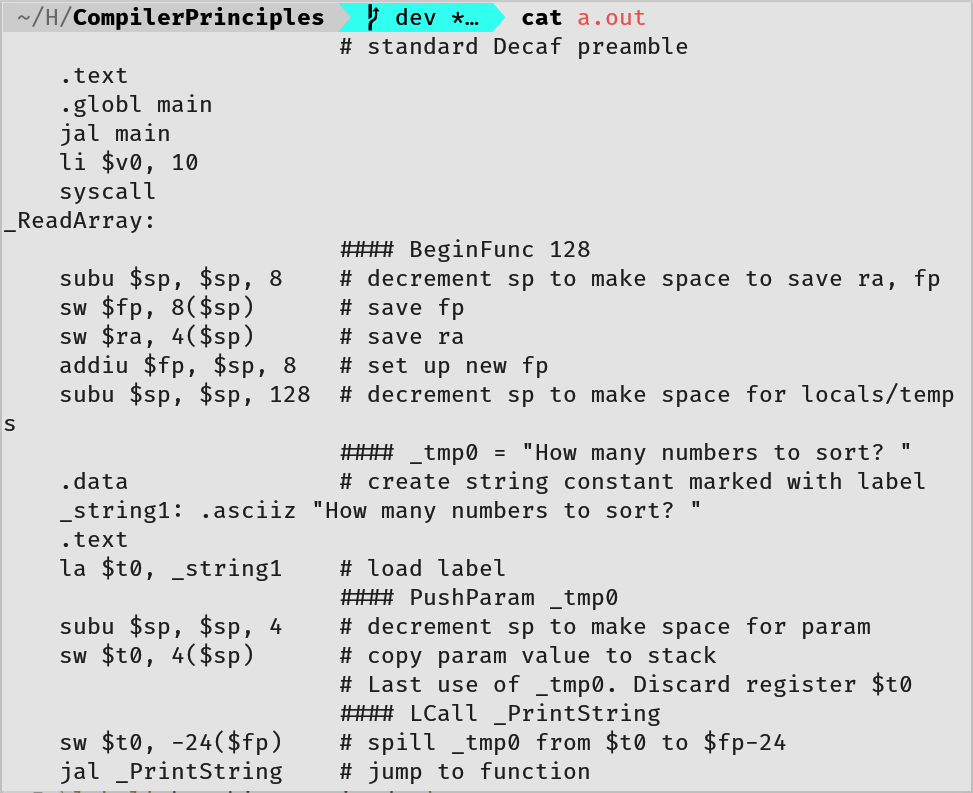
\includegraphics[width=0.74\linewidth]{asm.png}
    \caption{生成的汇编文件(部分)}
    \label{fig:asm}
\end{figure}

\par 由于之前在计算机组成原理课堂上实现的Mips CPU只能支持部分指令且不支持Ascii I/O,因此最终选择在Mips模拟平台Mars上进行模拟。模拟结果如图\ref{fig:simulate}所示。测试中,对于3, 6, 4, 2, 7, 12, 1, 0, 5, 10这10个数进行排序。从图中可以看出,排序结果正确,可以说明Decaf程序正确的完成了它的功能,编译器功能正常。
\begin{figure}[htpb]
    \centering
    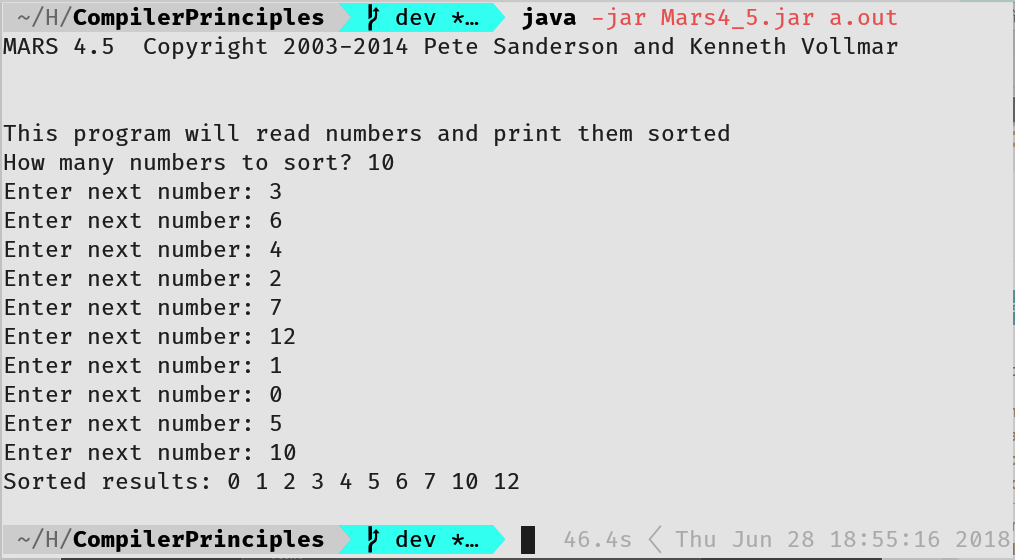
\includegraphics[width=0.8\linewidth]{simulate.png}
    \caption{Mars模拟编译后的程序运行结果}
    \label{fig:simulate}
\end{figure}

\chapter{实验心得}
\label{cha:shi_yan_xin_de_}
\par 在本次实验中,我借助flex,bison等工具从零开始制造了一个Decaf编译器,在这个过程中我收获了许多。首先,是对于编译器工作原理的理解,从前端到后端,从大体的流程框架到小的细节,我更加深入的理解了编译器是如何工作的,各个数据结构之间是如何转换与协同运作的。通过flex与bison的编写,我加深了对于课堂上所讲的源程序如何转换词汇表的理解
\par 除了编译原理有关的知识外,我还在编写的过程中对于C++的使用有了更深入一步的了解。经过反复的思考与设计,如何利用一个语言的特性来高效的设计编译器等。最重要的是,在这一个过程中,我体会到了如何完整的设计一个系统,使之可以无缝接合,正常工作,同又不至于耦合度过高,并具有一定的可扩展性。
\par 这次实验并不是一个十分完美的实验,还有许多可扩展的空间,如代码优化,寄存器优化,以及生成LLVM可识别的TAC等等。在时间有限的情况下,选择需要需要实现的重点内容对我来说也是一次十分宝贵的经验。这些所有的经验在将来的学习过程中也会由很大的帮助。

\appendix
{\let\clearpage\relax \chapter{程序使用方法}}
\label{cha:cheng_xu_shi_yong_fang_fa_}
\par 要编译本程序,需要在Linux环境下进行,并保证环境中安装有表\ref{tab:environment} 所示的同版本或更高版本的软件。在Makefile所在目录下运行make就可以自动编译了。
\par 生成的二进制文件为decafcc,dcc为使用bash脚本对其的包装。在使用时,推荐使用dcc这一包装。使用命令为\lstinline|./dcc <file>|,file为用于测试的decaf文件的路径。
\par 使用上述命令会生成\lstinline|tokens.out, ast.out, scope.out, tac.out, a.out|这5个文件,分别为词法分析结果,语法分析结果,符号表以及作用域分析结果,三地址码中间代码以及目标代码。使用cat命令可以直接在终端显示这些文件的内容。由于部分文件使用了linux颜色转义字符\footnote{\url{https://misc.flogisoft.com/bash/tip_colors_and_formatting}},因此使用文本编辑器打开极有可能不能正确显示,推荐在现代终端下使用cat命令进行输出。使用Mars 4.5及以上的版本打开a.out文件可以进行目标代码的模拟运行。

\chapter{测试用Decaf代码}
\label{cha:ce_shi_yong_decafdai_ma_}
\par 在本报告中使用的测试用decaf文件为一排序程序,程序如下。使用者也可以编写符合Decaf语法规范的程序进行测试。
\inputCodeSetLanguage{c++}
\begin{lstlisting}
int[] ReadArray() {
    int i;
    int num;
    int [] arr;
    int numScores;

    Print("How many numbers to sort? ");
    numScores = ReadInteger();
    arr = NewArray(numScores, int);
    i = 0;
    while (i < arr.length()) {
        Print("Enter next number: ");
        num = ReadInteger();
        arr[i] = num;
        i = i + 1;
    }
    return arr;
}

void Sort(int []arr) {
    int i;
    int j;
    int val;

    i = 1;
    while (i < arr.length()) {
        j = i - 1;
        val = arr[i];
        while (j >= 0) {
            if (val >= arr[j])
                break;
            arr[j + 1] = arr[j];
            j = j - 1;
        }
        arr[j + 1] = val;
        i = i + 1;
    }
}

void PrintArray(int []arr) {
    int i;
    i = 0;
    Print("Sorted results: ");
    while (i < arr.length()) {
        Print(arr[i], " ");
        i = i + 1;
    }
    Print("\n");
}


void main() {
    int[] arr;

    Print("\nThis program will read numbers and print them sorted\n");
    arr = ReadArray();
    Sort(arr);
    PrintArray(arr);
}
\end{lstlisting}

{\let\clearpage\relax \chapter{编译器源代码}}
\label{cha:bian_yi_qi_yuan_dai_ma_}

\par 各个文件的内容及作用如表\ref{tab:file}所示。
\begin{center}
    \begin{longtable}{r l r l}
        \caption{caption}
        \label{tab:file} \\

        \toprule
        \multicolumn{1}{c}{\textbf{文件}} &
        \multicolumn{1}{c}{\textbf{作用}} &
        \multicolumn{1}{c}{\textbf{文件}} &
        \multicolumn{1}{c}{\textbf{作用}} \\
        \cmidrule(lr){1-1} \cmidrule(lr){2-2}
        \cmidrule(lr){3-3} \cmidrule(lr){4-4}
        \endfirsthead

        \toprule
        \multicolumn{1}{c}{\textbf{文件}} &
        \multicolumn{1}{c}{\textbf{作用}} &
        \multicolumn{1}{c}{\textbf{文件}} &
        \multicolumn{1}{c}{\textbf{作用}} \\
        \cmidrule(lr){1-1} \cmidrule(lr){2-2}
        \cmidrule(lr){3-3} \cmidrule(lr){4-4}
        \endhead
        Doxyfile       & 文档生成配置文件       & ast\_stmt.cpp & 语法树语句结点实现\\
        Makefile       & Make文件               & ast\_stmt.h   & 语法树语句结点声明\\
        ast.cpp        & 语法树基类实现         & ast\_type.cpp & 语法树类型结点实现\\
        ast.h          & 语法树基类声明         & ast\_type.h   & 语法树类型结点声明\\
        ast\_decl.cpp  & 语法树声明节点实现     & codegen.cpp   & TAC代码生成器实现\\
        ast\_decl.h    & 语法树声明节点声明     & codegen.h     & TAC代码生成器声明\\
        ast\_expr.cpp  & 语法树表达式节点实现   & dcc           & 可执行文件decafcc包装\\
        ast\_expr.h    & 语法树表达式节点声明   & defs.asm      & decaf链接库\\
        errors.cpp     & 错误处理实现           & mips.cpp      & Mips指令生成器实现\\
        errors.h       & 错误处理声明           & mips.h        & Mips指令生成器声明\\
        flow.cpp       & CFG实现                & parser.h      & 语法分析器导出符号\\
        flow.h         & CFG声明                & parser.y      & 语法分析器bison文件\\
        hash.h         & 哈希表声明及实现       & printer.cpp   & 输出管理器实现\\
        list.h         & 链表声明及实现         & printer.h     & 输出管理器声明\\
        main.cpp       & 程序入口               & scanner.h     & 词法分析器导出符号\\
        scope.cpp      & 作用域声明             & scanner.l     & 词法分析器flex文件\\
        scope.h        & 作用域实现             & utility.h     & 工具类声明\\
        tac.cpp        & 三地址码实现           & utility.cpp   & 工具类实现\\
        tac.h          & 三地址码声明           & tags          & 索引标签\\
        \bottomrule
    \end{longtable}
\end{center}

\NewDocumentCommand{\appendixCode}{v m}{
    \noindent\par #1
    \inputCodeSetLanguage{#2}
    \lstinputlisting{../src/#1}
}
\par 部分关键源码如下(全部源码过于冗长,此处不再全部放出,详见源文件):
\appendixCode{scanner.l}{c++}
\appendixCode{parser.y}{c++}
\appendixCode{ast.h}{c++}
\appendixCode{codegen.h}{c++}
\appendixCode{mips.h}{c++}
\appendixCode{dcc}{bash}
\appendixCode{Makefile}{make}

\addcontentsline{toc}{chapter}{参考文献}
\nocite{*}
\bibliographystyle{plain}
\bibliography{report}

\vfill
{\tiny written by HuSixu \hfill powered by \XeLaTeX .}
\end{document}
